%
% teil2.tex -- Beispiel-File für teil2 
%
% (c) 2020 Prof Dr Andreas Müller, Hochschule Rapperswil
%
% !TEX root = ../../buch.tex
% !TEX encoding = UTF-8
%
\section{Einfacher Bruteforce Algorithmus
  \label{buch:paper:varalg:section:bruteforce}}
\rhead{Einfacher Bruteforce Algorithmus}
In der Bruteforce-Methode wird jede mögliche Variante durchprobiert,
um die beste Lösung zu finden. Dabei wird systematisch jede mögliche
Route durchlaufen und überprüft, wie lange die Strecke ist.
Ist die Strecke kürzer als die bisher kürzeste gefundene Route,
wird diese als neue optimale Lösung gespeichert.
\begin{figure}
    \centering
    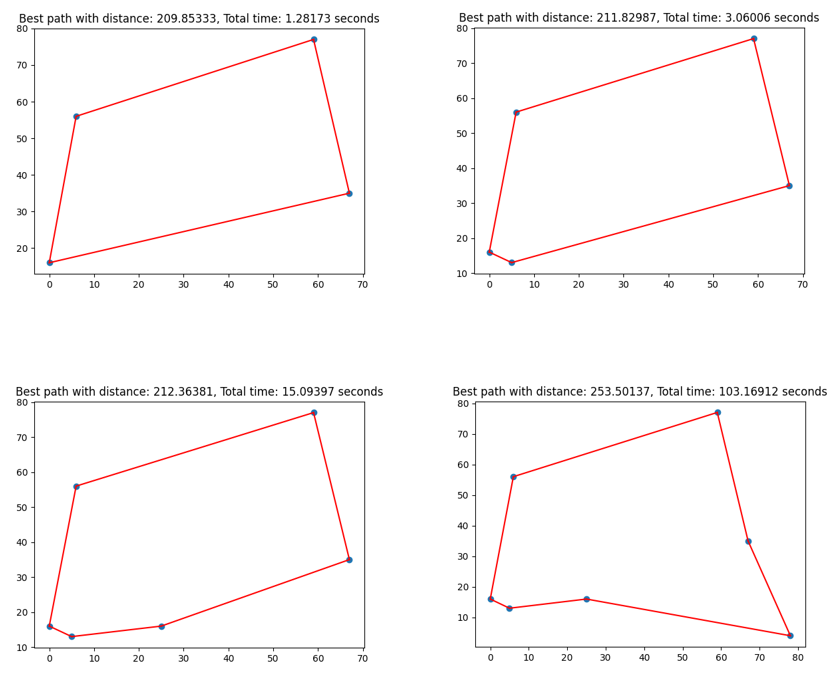
\includegraphics[width=0.8\textwidth]{papers/varalg/images/teil2/02BruteforceMethode.png}
    \caption{Resultate von verschiedenen Durchgängen mit steigender Anzahl von Städten.
        \label{fig:results_bruteforce}}
\end{figure}
Auf dem Bild \ref{fig:results_bruteforce} ist ersichtlich, dass der
Aufwand mit jedem weiteren Knoten exponentiell steigt. Anders
ausgedrückt, mit jeder weiteren Stadt gibt es mehr Varianten, die
durchprobiert werden müssen. Die Anzahl der Möglichkeiten lässt sich
mit der Formel \((n-1)!\) berechnen, wobei \(n\) die Anzahl der Städte ist.
Die Berechnung der verschiedenen Kombinationen lässt sich mit der
Formel
\begin{equation}
    L(\sigma)
    =
    \sum_{i=1}^{n-1} d(\sigma(i), \sigma(i+1)) + d(\sigma(n), \sigma(1))
    \label{eq:bruteforce_min_formula}
\end{equation}
beschreiben. Die Bedeutung der einzelnen Teile der Formel ist wie folgt:
\begin{itemize}
    \item \( L(\sigma) \) repräsentiert die Gesamtlänge der Rundreise.
    \item \( \sigma \) ist eine Permutation\footnote{
              Eine Permutation ist eine Anordnung von Objekten in einer bestimmten Reihenfolge.
              Zum Beispiel, wenn wir die Menge {1,2,3} haben, können daraus alle möglichen 
              Permutationen dieser Menge gebildet werden: 123, 132, 213, 231, 312, 321 
          }
          der Städte \( \{1, 2, \ldots, n\} \),
          wobei jede \( \sigma \) unterschiedliche Reihenfolge der Städte darstellt.
    \item \( d(i, j) \) ist die Funktion, welche die Entfernung zwischen der Stadt \( i \) und
          Stadt \( j \) zurückgibt.
\end{itemize}
\begin{beispiel}
    \label{buch:paper:varalg:subsection:bruteforce_calculate}
    Um zu verdeutlichen, wie die Formel \eqref{eq:bruteforce_min_formula}
    angewendet wird, folgt hier ein Beispiel. Für das Beispiel wird die Tabelle 
    \ref{tab:example_bruteforce_cities} genutzt.
    \begin{table}
        \centering
        \begin{tabular}{|c|c|c|c|c|}
            \hline
                & $A$ & $B$ & $C$ & $D$ \\ \hline
            $A$ & 0   & 10  & 15  & 20  \\ \hline
            $B$ & 10  & 0   & 35  & 25  \\ \hline
            $C$ & 15  & 35  & 0   & 30  \\ \hline
            $D$ & 20  & 25  & 30  & 0   \\ \hline
        \end{tabular}
        \caption{
            Beispieltabelle mit möglichen Distanzen zu den Städten, diese liest sich wie folgt:
            Die Distanz zwischen Stadt $B$ und $D$ beträgt 25.
        }
        \label{tab:example_bruteforce_cities}
    \end{table}
    In der Rechnung nutzen wir die Permutation $\sigma = (B, D, A, C)$.
    Diese setzen wir in die Formel ein:
    \begin{equation}
        L_1 = d(B, D) + d(D, A) + d(A, C) + d(C, B)
        =
        25 + 20 + 15 + 35 = 95
        \label{eq:bruteforce_min_formula_example}
    \end{equation}
    und erhalten für die Permutation die Gesamtlänge 95. Um die kürzeste Strecke zu finden,
    müssen alle möglichen Permutationen durchgerechnet werden. Die kürzeste Strecke ist dann
    das Optimum. 
\end{beispiel}
\subsection{Aufwand Bruteforce
    \label{buch:paper:varalg:subsection:bruteforce_efforts}}
\rhead{Aufwand Bruteforce}
Aus dem vorherigen Abschnitt \ref{buch:paper:varalg:section:bruteforce} ist 
ersichtlich, dass der Aufwand für die Berechnung der kürzesten Strecke exponentiell steigt.
Mit jedem weiteren Knoten gibt es mehr Permutationen, die berechnet und verglichen werden 
müssen. Aus den Testversuchen mit steigender Anzahl können die Resultate, welche in der 
Tabelle \ref{tab:bruteforce_tabelle_time} und der grafischen Abbildung \ref{fig:bruteforce_graph_time} 
dargestellt sind, erhalten werden. Daraus ist ersichtlich,
dass es bei 8 Städten einen Zeitaufwand von 17 Minuten erreicht.
% Tabelle
\begin{table}
    \centering
    \begin{tabular}{c d{4.4}}
        \toprule
        Punkte & \multicolumn{1}{c}{Zeit in Sekunden} \\
        \midrule
        1      & 0.6880                               \\
        2      & 0.6905                               \\
        3      & 0.7666                               \\
        4      & 1.2817                               \\
        5      & 3.0601                               \\
        6      & 15.0940                              \\
        7      & 103.1691                             \\
        8      & 1068.3832                            \\
        \bottomrule
    \end{tabular}
    \caption{Zeitverlauf mit steigender Anzahl von Städten}
    \label{tab:bruteforce_tabelle_time}
\end{table}
% Graph
\begin{figure}
    \centering
    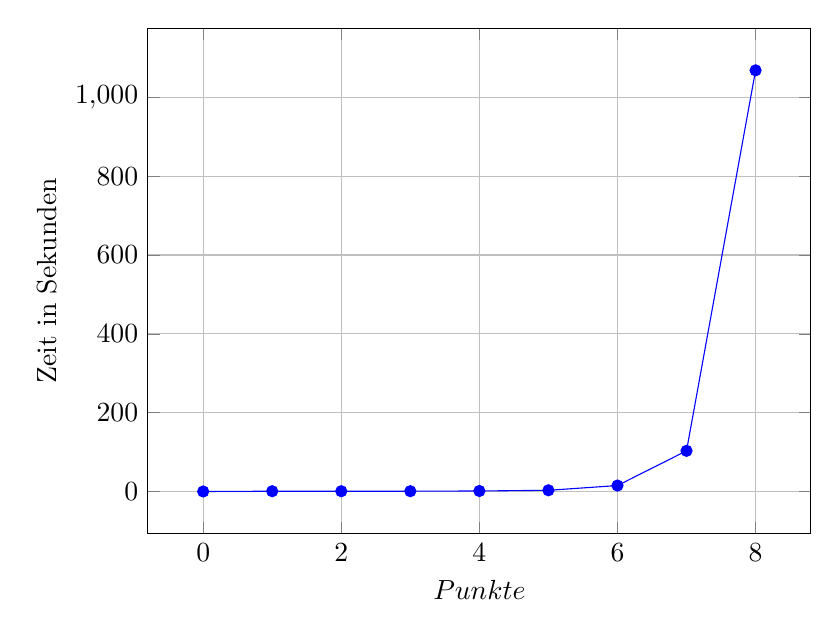
\begin{tikzpicture}
        \begin{axis}[
                xlabel=$Punkte$,
                ylabel=\text{Zeit in Sekunden},
                grid=major,
                width=10cm,
                height=8cm
            ]
            \addplot[
                color=blue,
                mark=*
            ] coordinates {
                    (0,0)
                    (1,0.6880)
                    (2,0.6905)
                    (3,0.7666)
                    (4,1.2817)
                    (5,3.0601)
                    (6,15.0940)
                    (7,103.1691)
                    (8,1068.3832)
                };
        \end{axis}
    \end{tikzpicture}
    \caption{Der Graph zeigt den Zeitverlauf mit steigender Anzahl von Städten}
    \label{fig:bruteforce_graph_time}
\end{figure}
